\apendice{Plan de Proyecto Software}

\section{Introducción}
En este anexo ser va a realizar un análisis de la planificación temporal junto con la viabilidad legal y económica del proyecto. 

\section{Planificación temporal}
\subsection{Introducción}
Para la planificación temporal se ha utilizado la metodología Scrum. El proyecto ha tenido dos fases muy diferenciadas. La primera fase está comprendida entre el Sprint 1 (13/10/2021) y el Sprint 10(04/03/2022), y se centra en el diseño y desarrollo del servicio web. La segunda fase comprendida entre el Sprint 11 (05/03/2022) y el Sprint Final (07/07/2022) se centra en la investigación, desarrollo e implementación de un sistema de recuperación de información musical. 

Estas dos fases se pueden diferenciar en las contribuciones del proyecto Fig.\ref{fig:A:contribuciones_del_proyecto}, ya que la segunda fase apenas tuvo impacto en el repositorio al desarrollarse desde Kaggle. 

\begin{figure}
    \centering
    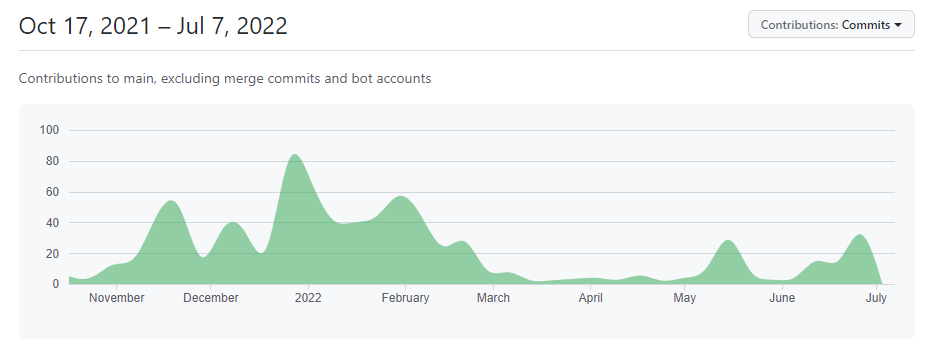
\includegraphics[width=\textwidth]{img/A/contribuciones.png}
    \caption{Contribuciones del Proyecto}
    \label{fig:A:contribuciones_del_proyecto}
\end{figure}

El proyecto se ha dividido en 5 Épicas:
\begin{itemize}
    \item \textbf{Spotify Frontend:} Esta épica contiene todas las tareas relacionada con el gestor de biblioteca / playlists / álbumes de Spotify. 
    \item \textbf{Database Frontend:} Esta épica contiene todas las tareas relacionadas con la interacción con la base de datos desde el Frontend. Además, se ha utilizado esta épica para la comunicacióon general con el backend. 
    \item \textbf{Backend Principal:} Esta épica contiene todas las tareas relacionada con el Backend NextJS, como la autenticación, transacciones de la base de datos, SSR, o comunicación con el analizador de tareas.
    
    \item \textbf{Analizador de Canciones:} Esta épica contiene todas las tareas relacionadas con el analizador de canciones, desde la investigación de técnicas y modelos, entrenamiento y experimentación con modelos hasta la implementación del backend. 
\end{itemize}

\subsection{Sprints}
Este apartado contine las distintas tareas organizadas por Sprints. No ha sido posible añadir una gráfica con el burndown debido a que Zenhub no permite generar el gráfico para los sprints anteriores a febrero. 

\subsubsection{Sprint 1}
\textbf{13/10/21 - 26/10/21}

\begin{itemize}
    \item Requisitos Funcionales. Coste inicial 1 punto, coste final  8 puntos. 
    \item Requisitos No Funcionales. Coste inicial  2 puntos, coste final 2 puntos.
    \item Buscar proveedores de Cloud. Coste inicial 2, Coste final 2.
    \item Diagrama de casos de uso. Coste inicial 3 puntos, coste final 8 puntos.
    \item Crear guía de estilo. Coste inicial 1 punto, coste final de 1 punto.
\end{itemize}


\subsubsection{Sprint 2}
\textbf{30/10/21 - 12/11/21}

\begin{itemize}
    \item Botón cambiar el Tema. Coste inicial 2, coste final 2.
    \item Diseño de la caché local. Coste inicial 2, coste final 2.
    \item Contexto de la API de Spotify, para que el cliente sea accesible desde todos los punto. Coste inicial de 2 puntos, coste final de 2 puntos. 
    \item Rutas Protegidas. Wrapper que impide a un usuario sin ciertas características acceder a ciertas rutas (por ejemplo /admin). Coste inicial 1 punto, coste final de 1 punto.
\end{itemize}


\subsubsection{Sprint 3}
\textbf{13/11/21 - 26/11/21}

\begin{itemize}
    \item Inicio de Sesión y Gestor de Cookies. Implementación del inicio de sesión y persistencia de credenciales en cookies. Coste inicial 8 puntos, coste final 8 puntos. 
    \item Caché Local. Se ha creado una caché local con DexieDB. Coste inicial 3, coste final 3. 
    \item Modal. Se ha creado un componente modal que contiene una vista anidad. Coste inicial 3, coste final 3.
    \item Track Card + Proxy de Carga. Se ha creado el componente carta que muestra una canción. Coste inicial 4, coste final 4. 
    \item Vista Genérica de Cartas. Se ha creado una vista genérica de cartas que pueda representar de forma eficiente cualquier tipo de tarjeta (canciones, álbumes, playlists o artistas). Coste inicial 8+5, coste final 8+5.
    \item Clientes REST Spotify y Lastfm. Coste inicial 2, coste final 2.
    \item Selector de Canciones para Playlist. Coste inicial 3, coste final 3.
    \item Implementación de los dátos homogéneos de Spotify. Coste inicial 2, Coste final 2. 
    
\end{itemize}



\subsubsection{Sprint 4}
\textbf{27/11/21 - 10/12/21}

\begin{itemize}
    \item Actualizar la versión de Typescript. Este cambio obligó a refactorizar los $catch$ ya que ahora necesitan estar tipados. Coste inicial 2, coste final 2.
    \item Configuración inicial de las acciones de Github para los tests de Jest. 
    \item Vista detallada de canciones. Coste inicial 3, coste final 3.
    \item Inicio de los filtros avanzados. 
    \item Inicio de la página de Inicio. Permite cargar las canciones y artistas favoritos del usuario. 
    \item Vista de artistas. Coste inicial 3, coste final 3. 
    \item Tarjeta de Artistas. Coste inicial 3, coste final 3. 
\end{itemize}


\subsubsection{Sprint 5}
\textbf{11/12/21 - 24/12/21}

\begin{itemize}
    \item Cambio en las proporciones de los botones para un diseño responsive. Coste inicial 1, coste final 1.
    \item Finalizado la integración de JEST con Github Actions. Coste inicial 2, coste final 2.
    \item Finalizados los filtros avanzados. Coste inicial 5, coste final 9.
\end{itemize}


\subsubsection{Sprint 6}
\textbf{11/12/21 - 24/12/21}

\begin{itemize}
    \item Terminar Home Page, integrando las distintas vistas. Coste inicial 2, coste final 13.
    \item Caché Manager. Implementación de la fachada como Hook de react. Coste inicial 5, coste final 5.
    \item Mejorar el rendimiento de la fachada. Las peticiones se realizan en paralelo. Coste inicial 
    \item Sistema de Notificaciones Genérico. Coste inicial 5, coste final 5.
    \item Caché de Notificaciones. Coste inicial 5, coste final 5. 
    \item Vista de Playlist. Coste inicial 5, coste final 5.
    \item Implementación de JWT. Coste final 5, costes final 5.
    \item Implementación de Vista de Estadísticas. Coste inicial 8, coste final 8.
    \item Detalles de Playlist. Coste inicial 5, coste final 5.
\end{itemize}


\subsubsection{Sprint 7}
\textbf{8/01/22 - 21/01/22}

\begin{itemize}
    \item Estado de la Fachada mediante un spinner. Coste inicial 2, coste final 2.
    \item Menú de navegación de Escritorio. Coste inicial 5. Coste final 8.
    \item Barra de navegación móviles. Coste inicial 5, coste final 5.
    \item Página de Opciones. Coste inicial 8. Coste final 8.
    \item Reproductor / Suena Ahora. Coste inicial 8, coste final 8.
    \item Selector de lenguaje. Coste inicial 4, coste final 4.
\end{itemize}

\subsubsection{Sprint 8}
\textbf{22/01/22 - 04/02/22}
\begin{itemize}
    \item Cliente de la base de datos. Coste inicial 4, coste final 4.
    \item Implementación de transacciones de etiquetas. Coste inicial 3, coste final 3.
    \item Exposición de las etiquetas mediante API REST. Coste inicial 3, coste final 3.
    \item Documentar la especificación de la API mediante OpenAPI. Coste inicial 1, coste final 1.
    \item Test de las APIs mediante Cypress. Coste inicial 3, coste final 3. 
    \item Solucionar el cambio de la URL de la API al cambiar el idioma. Coste inicial 1, coste final 1.
    \item Solucionar problemas de re-renderizado indeseados. Coste inicial 3, coste final 3.
    
    \item Vista de álbumes. Coste inicial 3, coste final 3.
\end{itemize}







\subsubsection{Sprint 9}
\textbf{05/02/22 - 18/02/22}
\begin{itemize}
    \item Detalles de álbumes. Coste inicial 2, coste final 2. 
    \item Gestor de Álbumes. Coste inicial 8, coste final 8.
    \item Editor de etiquetas de álbumes. Coste inicial 3, coste final 3.
    \item Investigar sobre técnicas de clasificación musical. Coste inicial 4, coste final 4.
    \item Demo de clasificador con Keras y Gtzan. Coste inicial 8, coste final 8.
    \item Página de Búsqueda. Coste inicial 5, coste final 5.
    \item Investigar técnicas y resultados de audio augmentation. Coste inicial 2, coste final 2.
    \item Ocular el fondo del modal con CSS. Coste inicial 1, coste final 1.
\end{itemize}


\subsubsection{Sprint 10}
\textbf{19/02/22 - 04/03/22}
\begin{itemize}
    \item Entrenar GTZAN a partir de modelos preentrenados. Coste inicial 5, coste final 5.
    \item Añadir vistas anidadas en los detalles. Coste inicial 8, coste final 8.
    \item Desarrollo de una aplicación en Node que permita descargar canciones de la API de Spotify. Coste inicial 3, coste final 5.
    \item Extensión del conjunto de datos GTZAN con 200 canciones más por cada género. Coste inicial 5, coste final 8. 

\end{itemize}

\subsubsection{Sprint 11}
\textbf{12/03/22 - 01/04/22}

\begin{itemize}
    \item Normalización de Playlist mediante Node. Coste inicial 3, coste final 3.
    \item Modelado del Dataset que incluya subgéneros. Coste inicial 1, coste final 1.
    \item Obtención de las etiquetas de Discogs. Coste inicial 2, coste final 2.
    \item Investigar Gtzan con técnias de clustering mediante DB SCAN y Kmeans. Coste inicial 2, coste final 2.
    \item Herramienta que extraiga los MFCCs y los almacene en fichero .npy. Coste inicial 2, coste final 2.
    \item Creación del Ludwig Dataset. Coste inicial 13, coste final 13.
\end{itemize}


\subsubsection{Sprint 12}
\textbf{2/04/22 - 22/04/22}
\begin{itemize}
    \item Implementación de una OVA para mejorar el resultado del clasificador en Ludwig. Coste inicial 13, coste final 13.
    \item Eliminar Reggae como género principal. Coste inicial 1, coste final 1.
    \item Implementar una arquitectura OVO de 32 CNNs para mejorar el rendimiento del clasificador. Coste inicial 3, coste final 8.
    \item Implementar Adaboost para mejorar el rendimiento. Coste inicial 3, coste final 3.
    \item Clasificar la salida de CNN mediante SVM para mejorar el rendimiento. Coste inicial 3, coste final 3.
    \item Entrenar todos los subgéneros. Coste inicial 5, coste final 5.
    \item Entrenar una OVA como clasificador de estados de ánimo. Coste inicial 8, coste final 8.
    
    \item Iniciar el Backend de MIR. Coste inicial 2.
    
\end{itemize}

\subsubsection{Sprint 13}
\textbf{23/04/22 - 06/05/22}
\begin{itemize}
    \item Implementar el motor de inferencia basado en ONNX. Coste inicial 5, coste final 5.
    \item Terminar el Backend de MIR. Coste final 8.
    \item Mejorar el rendimiento mediante inferencia en bloque. Coste inicial 3, coste final 3. 
    \item Configurar la integración continua de GCP Run par que publique el Backend MIR. Coste inicial 2, coste final 2.
    \item Sistema de recomendación basado en contenidos. Coste inicial 8, coste final 8.
    \item Sistema de recomendación colaborativo. Coste inicial 8, coste final 8.
\end{itemize}

\subsubsection{Sprint 14}
\textbf{07/05/22 - 20/05/22}
\begin{itemize}
    \item Integración Backend MIR con Frontend. Coste inicial 12, coste final 16.
    \item Cuantización de Modelos para reducir el consumo de memoria. Coste inicial 1, coste final 1.
    \item Internacionalización completa al castellano. Coste inicial 8, coste final 8. 
\end{itemize}


\subsubsection{Sprint 15}
\subsubsection{Sprint 14}
\textbf{21/05/22 - 03/06/22}
\begin{itemize}
    \item Desarrollo de los conceptos teóricos. Coste inicial 8, coste final 8.
    \item Protección del backend MIR mediante un código secreto. Coste inicial 3, coste final 3.
    \item Actualización de Estadísticas para incluir estados de ánimo. Coste inicial 3, coste final 3.
\end{itemize}


\subsubsection{Sprint Final}
\textbf{03/06/22 - 07 / 07 / 22}
\begin{itemize}
    \item Documentación de técnicas y herramientas. Coste inicial 8, coste final 8.
    \item Documentación de aspectos relevantes. Coste inicial 8, coste final 8.
    \item Documentación de Objetivos. Coste inicial 1, coste final 1.
    \item Documentación de Introudcción y Abstract. Coste inicial 1, coste final 1.
    \item Creación de Docker Compose. Coste inicial 4, coste final 4.
    \item Crear página de inicio. Coste inicial 4, coste final 4.
    \item Finalizar anexos de diseño y requisitos. Coste inicial 8, coste final 8.
    \item Crear una vista de sistema mediante Figma. Coste inicial 2, coste final 2.
    \item Documentación del Plan de Proyecto. Coste inicial 8, coste final 8.
\end{itemize}



\section{Estudio de viabilidad}

En este apartado se va realizar un estudio sobre la viabilidad económica y legal del proyecto, teniendo en cuenta distintos apartados como los

\subsection{Viabilidad económica}

El proyecto no es económicamente viable ya que los términos y condiciones de Spotify \cite{Spotify_terms:online} y LastFM \cite{A:Last_APITerms18:online}. Estos servicos solo permiten utilizar la API pública para \textbf{uso personal}, por lo que no se puede monetizar.

\subsubsection{Costes}

En esta sección se van a desglosar y analizar los distintos costes del proyecto.

\textbf{Costes de Hardware}

Los únicos costes hardware son un ordenador portátil junto con sus periféricos.

Suponiendo que la vida útil de un ordenador portátil son 6 años podemos estimar su coste amortizado durante el primer año. Estos costes están desglosados en \ref{A:tab:hardware}

\begin{table}[H]
\centering{%

    \begin{tabular}{@{}lll@{}}
    \toprule
    Concepto               & Coste (€) & Amortización (€) \\ \midrule
    Portátil y Periféricos & 850       & 631              \\ \midrule
    Total                  & 850     & 631                 \\ \bottomrule
    \end{tabular}%
    }
    \caption{Costes Hardware}
    \label{A:tab:hardware}
\end{table}

\textbf{Costes Fijos de Software}

En este apartado \ref{A:tab:fijos} se van a analizar los costes anuales de los distintos servicios y suscripciones. 

\begin{table}[H]
\centering{%
    \begin{tabular}{@{}lll@{}}
    \toprule
    Concepto               & Coste (€) & Amortización (€) \\ \midrule
    Vercel\footnote{Alojamiento de la Web} & 240       & 163.7            \\
    Codacy & 170       & 113           \\ 
    Github Premium &   48     & 32.2           \\ 
    Github Copilot & 120      & 163.7            \\ \midrule
    Total                  & 578    & 488.4               \\ \bottomrule
    \end{tabular}%
    }
    \label{A:tab:fijos}
    \caption{Costes Fijos}
\end{table}

\textbf{Costes por Usuario}

Según los análisis de Google Cloud Platform, el coste medio por usuario por usuario para cada uno de los servidores webs son unos 13.26 céntimos al mes, siendo el servidor web de análisis de canciones el más cara de mantener por los altos tiempos de ejecución y consumos de memoria. 

AWS DynamoDB tiene un coste mensual de 0.072 céntimos por cada unidad de lectura y escritura en la base de datos, y un coste de 0.283 céntimos por cada GB/mes. Se estima que es necesaria 1 unidad de lectura y escritura por cada 10000 usuarios. Cada canción almacenada tiene un tamaño medio de 412 Bytes y cada usuario almacena de media 1.2KB en etiquetas. \\
Serían necesarios 200 millones de usuarios (más usuarios que suscriptores de Spotify \cite{A:spot_subs}) o 625 millones de canciones almacenadas. Como es prácticamente imposible alcanzar estos números de usuarios o canciones, se ha decidido obviar el coste del almacenamiento debido a que el uso comercial entra dentro del plan gratuito de AWS. 

Podemos estimar que el coste por usuario es de unos \textbf{14 céntimos al mes}. Además, a medida que se analicen más canciones, es posible que el coste se vea reducido debido al aumento de lecturas en la base de datos y el menor uso del analizador de canciones. 

\textbf{Costes Personal}

Para este coste se va a tener en cuenta el coste de un único empleado encargado del desarrollo, mantenimiento y soporte de usuario de la página web hasta que se decida dejar de dar soporte al servicio. 

En este caso se ha escogido un suelo base bruto de 21.000 euros, considerando el salario de un desarrollador junior fullstack sin apenas experiencia, que ha sido desglosado en \ref{A:salario}

\begin{table}[H]
    \centering{%
    \begin{tabular}{ll}
    \hline
    Concepto                                                                                                         & Coste (€) \\ \hline
    Salario Mensual Neto (12 pagas) &  1.425,4   \\
    Retenciones IRPF & 2.562,2 \\
    Cuotas Seguridad Social &  1.333,5 \\
    \hline
    Total & 21.000,0
    \\ \hline
    \end{tabular}%
    }
    \label{A:salario}
    \caption{Desglose Coste anual del Webmaster}
\end{table}

\textbf{Otros Costes}

La tabla \ref{A:otros_costes} contiene otros costes que han aparecido a lo largo del proyecto. 
\begin{table}[H]
    \centering{%
    \begin{tabular}{ll}
    \hline
    Concepto                                                                                                         & Coste (€) \\ \hline
    3 USBs &  14,5  \\
    Memoria & 23,5       \\
    \hline
    Total & 38,0\\
    \hline
    \end{tabular}%
    }
    \label{A:otros_costes}
    \caption{Coste anual del Webmaster}
\end{table}
\textbf{Coste Primer Año}

La tabla  \ref{A:coste_ano_1} contiene el coste del proyecto durante el primer año. 

\begin{table}[H]
    \centering{%
    \begin{tabular}{ll}
    \hline
    Concepto                                                                                                         & Coste (€) \\ \hline
    Salarios &  21.000,0   \\
    Licencias & 488,4 \\
    Hardware & 631 \\
    20 Usuarios & 3,33 \\                                                                 \hline
    Total & 22122.73 \\ 
    \hline
    \end{tabular}%
    }
    \label{A:coste_ano_1}
    \caption{Coste durante el primer año}
\end{table}

\subsection{Viabilidad legal}

En esta sección se va a analizar las distintas licencias de las dependencias, así como términos y condiciones de las APIs que hemos utilizado. 

\subsubsection{Api de Spotify}
La api de Spotify detalla sus términos y condiciones en \cite{A:SpotifyTerms:online}. Los términos más importantes están reflejados en la tabla \ref{tab:A:spotify_terms}.

\begin{table}[h]
    \resizebox{\textwidth}{!}{%
    \begin{tabular}{@{}ll@{}}
        \toprule
        Condición                                                                                                                                                  & Estado \\ \midrule
        Uso No Comercial                                                                                                                                           &   \checkmark   \\
        \begin{tabular}[c]{@{}l@{}}No se almacenan datos de Spotify \\ que puedan quedarse obsoletos\end{tabular}                                                  & \checkmark        \\
        \begin{tabular}[c]{@{}l@{}}Los resultados tienen en cuenta el mercado\\ del usuario / no permite a usuarios saltarse restricción geográficas.\end{tabular} & \checkmark        \\
        \begin{tabular}[c]{@{}l@{}}La plataforma cumple con las recomendaciones\\  de la guía de diseño de Spotify\end{tabular}                                    &\checkmark         \\
        No se modifican los metadatos de Spotify                                                                                                                   & \checkmark        \\
        No se utiliza la API para uso malicioso                                                                                                                    & \checkmark        \\
        No se daña la imagen de Spotify                                                                                                                            & \checkmark        \\
        Incumplimiento de la propiedad intelectual                                                                                                                 & \checkmark        \\
        \begin{tabular}[c]{@{}l@{}}Se oculta la implementación de características $Premium$ a\\
        usuarios que no son suscriptores\end{tabular}                      &  \checkmark       \\ 
        No se cachean los resultados de la API & \textbf{\~}\\

        \bottomrule
    \end{tabular}%
    }
    \label{tab:A:spotify_terms}
    \caption{Términos y Condiciones más importantes de la API de Spotify}
\end{table}


El punto más interesante es la sección IV apartado 3b, que prohíbe el uso de caches. Si detallamos este punto se puede observar como únicamente se permite el uso de cachés si \textbf{se utilizan para el rendimiento}, \textbf{son temporales}. SpotMyFM cumple con ambos casos de uso.

\subsubsection{Api de LastFM}

Los términos y condiciones de la API pública de LastFM pueden encontrarse en \cite{A:Last_APITerms18:online}.
En este caso, se pueden resaltar los términos y condiciones en la siguiente tabla \ref{A:last_terms}.

\begin{table}[H]
    \centering{%
    \begin{tabular}{ll}
    \hline
    Condición                                                                                                           & Estado \\ \hline
    Se acredita el origen de los datos a LastFM                                                                         &  \checkmark      \\
    Uso No Comercial                                                                                                    &  \checkmark       \\
    No se licencian los datos de LastFM                                                                                 &    \checkmark    \\
    \begin{tabular}[c]{@{}l@{}}No se modifican los datos de LastFM de\\ manera que dañe la imagen de marca\footnote{No se han modificado los datos de ninguna manera.}\end{tabular} &  \checkmark      \\ \hline
    \end{tabular}%
    }
    \label{A:last_terms}
    \caption{Términos y Condiciones más importantes de la API de LastFM}
\end{table}
En este caso se han cumplido con todos los requisitos que especifican los términos y condiciones de la API. 

\subsubsection{Licencias Software}
Una licencia software es una definición legal vinculante que indica los límites y condiciones para el uso de cada una de las dependencias. Cada dependencia puede tener un tipo de licencia distinto, por lo que es necesario revisar si algunas de las licencias es incompatible con el proyecto. 

Las licencias de cada una de las dependencias han sido detalladas en \ref{tab:A:Licencias}. Todas las licencias admiten los distintos usos que va a tener el producto.  

\begin{table}[H]
    \centering
    \begin{tabular}{ll}
    \hline
        Dependencia & Licencia \\
         Babel & MIT \\
         Cypress & MIT y Apache \\
         Jest & MIT \\
         npmcli & ISC \\
         popperjs & MIT \\
         @uiball/loader & MIT \\
         axios & MIT \\
         base64 & MIT \\
         dexie & Apache 2.0 \\
         dotenv & BSD-2-Clause \\
         Framer Motion & MIT \\
         js-cookies & MIT \\
         jsonwebtoken & MIT \\
         lodash & MIT \\
         next & MIT \\
         next-translate & MIT \\
         pretty-ms & MIT\\
         react-device-detect & MIT \\
         react-dom & MIT \\
         react-icons & MIT \\
         react-switch & MIT \\
         react-is & MIT \\
         react-toastify & MIT \\
         react-use & MIT \\
         recharts & MIT \\
         spotify-web-api-js & MIT \\
         spotify-web-api-node & MIT \\
         styled-components & MIT \\
         tiny-async-pool & MIT \\
         twin.macro & MIT \\
         estlint & MIT \\
         ONNX & Apache 2.0 \\
         FastAPI & MIT \\
         Tensorflow & Apache 2.0 \\
         Python & PSFN\footnote{Python Software Foundation License, compatible con GPL} \\
         
         
    \hline
    \end{tabular}
    \caption{Licencias}
    \label{tab:A:Licencias}
\end{table}
